\documentclass{article}

\usepackage[main=english,vietnamese]{babel}
\usepackage[T1]{fontenc}
\usepackage[utf8]{inputenc}
\usepackage[sexy]{evan}
\usepackage{matchsticks}
\usepackage{wrapfig}
\usepackage{listings}

\newtheorem{hint}{Hint}

\title{Proof by Contradiction - Part 1}
\author{Nghia Doan}
\date{\today}

\begin{document}

\maketitle

In this article, when approaching a problem, we start by assuming that some fact or statement is true.
Next, we demonstrate that the consequences of this assumption lead to inconsistency.
Therefore, we can conclude that the original assumption is incorrect.
This approach of thinking about a problem is called \textit{a proof by contradiction}.

\begin{example*}[Example 1]
    Together, 5 soccer players together scored 14 goals, with every player scoring at least 1.
    Prove that at least 2 of them scored the same number of goals.
\end{example*}

\begin{remark*}
    Let say if a student comes up with a solution like this:
    \textit{"If the first player scored 1 goal, the second player scored 2, and so on,
    then the total number of goals would be 15, which is more than 14. Problem solved.”}

    What's wrong with this? The main issue with this argument is that
    it deals with \textit{one specific scenario}: 1 goal by the first player, 2 by the second, and so on.
    What if no one scored exactly 1 goal, or the third player scored 7?
    \textbf{We cannot use one case to prove the entire problem.}
\end{remark*}

\begin{soln}
    \textit{Proof by contradiction} provides a simple framework for a proof.
    Let's start by \textbf{assuming that no two players scored the same number of goals.}
    If we order the players by their scores, then the first player scored \textit{at least 1},
    the second one \textit{at least 2}, the third one \textit{at least 3}, the fourth one \textit{at least 4},
    and the fifth one \textit{at least 5}.
    (Note that we never claim that a player achieved some specific score: we always use the word \textit{at least}.)
    The players altogether scored at least 1 + 2 + 3 + 4 + 5 = 15. However, the total score is 14.
    \textbf{This contradiction} proves that \textit{there must have been at least two players with the same score.}
\end{soln}

\begin{example*}[Example 2]
    The parliament of a certain country is formed by representatives from 8 provinces.
    Fifty of these parliamentarians decide to form a committee.
    Prove that this committee will include 8 people from the same province or people from all 8 provinces.
\end{example*}

\begin{soln}
    \textit{To the contrary, assume that we were able to find a group of 50 parliamentarians} such that
    no more than 7 people are from the same province and at least 1 province is not represented.
    Then, since 1 province is not there, at most 7 provinces are included.
    At the same time, each province is represented by at most 7 parliamentarians.
    So, there should be no more than $7 \times 7 = 49$ representatives altogether.
    This conclusion \textit{contradicts the fact} that the group has 50 people.
    Therefore, such a committee cannot be formed.
\end{soln}

\newpage

\begin{example*}[Example 3]
    Can you find five odd numbers whose sum is 100?
\end{example*}

\begin{soln}
    \textit{Let assume that you can}, then after subtracting one of the numbers from 100.
    We know that the sum of any two odd numbers is an even number,
    so the sum of any two three numbers is an odd number,
    thus the sum of any two four numbers is an even number,
    and finally the sum of any two five numbers is an odd number.
    This contradicts the fact that 100 is an even number.
\end{soln}

\begin{example*}[Example 4]
    Each node of a square grid is coloured either black or white.
    Prove that it is possible to find 3 nodes of the same colour that are located at the vertices of a right triangle.
\end{example*}

\begin{soln}
    \textit{Let assume the opposite,} so no right triangle can have all three vertices with the same colour.
    Let $\triangle ABC$ be a right triangle such that $A$ and $B$ with the same colour, while $C$ has the other.
    Since we can always rorate the grid, let $\triangle ABC$ be coloured as shown in the diagram below.

    \begin{center}
        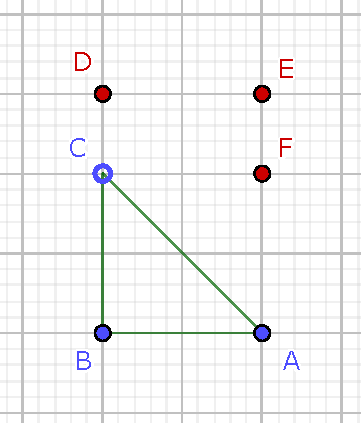
\includegraphics[width=4.5cm]{./svg/pdf/sc-23-ms-2-e4.pdf}
    \end{center}
    
    Now, consider points $D, E,$ and $F$ temporarily shown as red nodes.
    None of them can be the same colour of $A$ (and $B$).
    Thus all of them has the same colour and they form a right triangle with three vertices of the same colour.
    This contracicts the assumption, thus it is possible to find 3 nodes of the same colour
    that are located at the vertices of a right triangle.
\end{soln}

\begin{example*}[Example 5]
    A closed path is made up of 11 line segments. Can one line, not containing a vertex of the path, intersect each of its segments?
\end{example*}

\begin{soln}
    No, it cannot. Suppose we did have such a line.
    If we trace the path, each time we intersect the given line
    we pass from the half-plane on one side of the line to the half-plane on the other side
    (any line divides a plane into two half-planes)
    Since the path is closed, we begin and end on the same side of the line.
    The sides of the line alternate, so the close path would have evenly many vertices.

    This contradicts the fact that the close path has 11 segments.
\end{soln}
    
\end{document}